\section{A fejlesztés fogalmai}

\subsection{A \textit{GTK+} objektum-orientáltsága}

Ebben a fejezetben arra próbálunk mélyebben is rávilágítani, hogy a \textit{GTK+} ugyan \textit{C} nyelven íródott, de számos az objektum-orientált nyelvek esetén megszokott terminológiát használ, sőt ezeket a nyelvi eszközök adta mértékben meg is valósítja. Ezért az objektum-orientált fejlesztés fogalmait, kifejezéseit joggal használjuk még akkor is, ha \textit{GTK+} nyelvű fejlesztésről esik szó.

Azzal együtt, hogy az objektum-orientált mechanizmusokat nyelvi szinten a \textit{C} nem, csak a \textit{C++}, illetve a \textit{Python} támogatja lehetséges ezekkel élni ezen változat esetén is. Lássuk mik lennének ezek és hogyan válik lehetővé alkalmazásuk a \textit{GTK+} esetén.

\subsubsection{Egységbezárás}
\index{egységbezárás}
\index{GObject@\texttt{GObject}}

Az objektum-orientált alapelvek közül \textit{C} nyelven nem könnyen biztosíthatóról beszélünk, ugyanakkor a \textit{GTK+} megteszi, amit ebben a tekintetben megtehető. Az adatstruktúrákat -- jelen esetben \textit{widget}eket -- és az azokon műveleteket végző függvényeket a lehetőségekhez mérten egységkén t kezeli, valamint elrejti őket a külvilág elől.

A \textit{GTK+} minden saját makrót/függvényt \texttt{GTK}/\texttt{gtk} prefixszel lát el (a \textit{GLib} esetén ez pusztán csak egy kis, illetve nagy \texttt{g} betű). Egy adott részterület -- például egy \textit{widget} -- saját ``névtérrel'' is rendelkezhet, azaz újabb prefixet vezethet be\footnote{a \textit{GtkWindow} típushoz tartozó függvények prefixe \texttt{gtk} helyett \texttt{gtk\_window}}. Ezeket egymástól, illetve a ``valódi'' funkciót jelölő nevektől \texttt{\_} (aláhúzás) jellel választják el. A \textit{C++} wrapper esetén -- kihasználva a kézenfekvő nyelvi lehetőséget -- a prefixek szerepét természetesen a névterek, illetve az osztályok veszik át\footnote{a \textit{Window} típus a \textit{gtkmm} esetén \texttt{Gtk} névtéren belül szereplő \texttt{Window} nevű osztály}.

\index{átlátszatlan mutató}
Ezen prefixelt makrók/függvények első paramétere minden esetben a prefix által meghatározott típusú objektum, elősegítve ezzel is ezen függvények, illetve az általuk kezelt objektumok egy egységként való kezelését. A privát adatok külvilág elöl való elrejtésére a \textit{C} nyelven erre a célra széles körben alkalmazott átlátszatlan mutatókat\footnote{a módszer egyebek mellett \textit{pimpl} (\textit{pointer to implementation idiom}) néven is ismert} (\textit{opaque pointer}) használja a \textit{GTK+}, ami lehetővé teszi az objektum által használt adatszerkezetek, implementációs módszerek elfedését a publikus interfész használó kódok elöl.

\subsubsection{Öröklés}
\index{öröklés}
\index{GObject@\texttt{GObject}}
\index{gtkmm@\textit{gtkmm}}
\index{PyGObject@\textit{PyGObject}}

Megoldott a \textit{widget}ek egymásból történő származtatása, sőt felhasználói widgetek is definiálhatóak a már meglévőekre támaszkodva. Az kód újrahasznosítását jól mutatja az a tény, hogy a \texttt{GObject} osztály -- mely önmagában is számos hasznos funkcióval rendelkezik -- minden \textit{widget}, illetve számos  más a \textit{GTK}-ban használt nem vizuális elemnek őse. Meg kell jegyezni, hogy a \textit{gtkmm}, illetve a \textit{PyGObject} esetén -- lévén ezen esetekben az objektum-orientáltságot támogatja mag a nyelv -- természetesen a származtatás egy nagyságrenddel egyszerűbb, de mintapéldákat felhasználva némi rutinnal a \textit{GTK+} esetén sem igényel különösebb erőfeszítést.

A \textit{widget}ek öröklési fájáról már itt érdemes megjegyezni, nem csupán két szintű, vagyis azzal együtt, hogy a \textit{GObject} típus a fa csúcspontja, de nem az egyetlen csomópontja. A hasonló funkcionalitású, következésképp rendszerint hasonló megjelenésű \textit{widget}ek (\ref{fig:widgetinheritance}) értelemszerűen egymásból származnak. Ez még a leghétköznapibb esetekben is igaz. A számok kezelésére is alkalmas \textit{widget} (\textit{spin button}) őse az egyszerű, egy sornyi szöveg befogadására alkalmas beviteli mezőt megvalósító \textit{widget} (\textit{entry}).

\includetwingraphics
{Egysoros beviteli mező}
{entry}
{entry.png}
{Számbeviteli mező}
{spinbutton}
{spinbutton.png}
{Öröklés hasonló funkciójú \textit{widget}ek között}
{widgetinheritance}

A mechanizmus további előnye az interfészek\footnote{a kifejezés alatt a \textit{Java} nyelv interfész, illetve a \textit{C++} absztrakt osztálya értendő} kialakításának lehetősége. A \textit{GTK+} a 3-as főverziót megelőzően törekedett arra, hogy a különböző \textit{widget}ek azonos funkciót megvalósító részeit (kattintható, szerkeszthető, görgethető elemek) egységes programozási felületen keresztül érhetjük el.

\subsubsection{Polimorfizmus}
\index{GObject@\texttt{GObject}}
\index{fordítási idejű típusellenőrzés}

Hasonlóan az öröklődéshez -- pusztán nyelvi szinten -- itt sem érhető el teljek körű megoldás \textit{C} nyelv esetén. Ugyanakkor a fő momentum, vagyis a származási hierarchia egyes osztályainak specifikus viselkedése egy adott funkciót megvalósító metódusok tekintetében elérhető. A \textit{widget}eket leíró struktúrákban ugyanis a származtatott osztályokból felülírhatóak az egyes funkciókat implementálható függvények mutatói\footnote{ami hasonló eredményre vezet, mint a \textit{C++} \texttt{virtual} kulcsszavának használata esetén}. Az így létrejövő többalakúság bár közel sem tökéletes, ám számos gyakorlati problémát megold.

Ezen felül a \textit{GTK+} minden \textit{widget}típushoz -- mondhatni osztályhoz -- definiál egy-egy makrót, melyek segítségével futásidőben ellenőrizhető egy adott \textit{widget} tényleges típusa, hasonlóan ahhoz, amire a \textit{dynamic\_cast} használata ad lehetőséget a \textit{C++}-ban. Azt a mechanizmust, melynek révén lehetővé válik a \textit{GTK+}-ban a futás idejű típusellenőrzés, a már említett \texttt{GObject} osztály implementálja, az ebből származó saját osztályainknak nem csupán lehetséges, de szükséges is a használata.

\subsection{A \textit{GTK} alapfogalmai}

\subsubsection{Widget}
\index{widget@\textit{widget}}

A fogalmat egyrészt, mint gyűjtőfogalmat használjuk a grafikus felhasználói felületek programozása során a felhasználó felületek egyes grafikai elemeinek megnevezésére\footnote{ebben az értelemben a ''window gadget'' kifejezés rövidítése}, mint amilyen például egy rádiódomb, egy szövegbeviteli mező, vagy akár egy kép.  Másrészről a \texttt{GtkWidget} minden -- ez előbbi értelemben vett \textit{widget} -- ősosztálynak a neve is -- még ha az öröklődés a \textit{C} nyelvben nem is létezik -- melyből minden egyes elem származik.

A \texttt{GtkWidget} osztály, mint a \textit{widget} fogalom objektum-orientált leképezése a felhasználó felület egyes elemeinek tulajdonságait, illetve az azokhoz kapcsolódó műveleteket zárja egységbe, biztosítva egyúttal az általa implementált funkciók újrahasznosíthatóságát éppúgy, mint a felülbírálhatóságukat. Kérdés persze, hogy ezen általánosság mögött pontosan mi is rejtőzik.

\subsubsection{Tulajdonságok}
\index{widget@\textit{widget}!tulajdonságok}

A mindennapi felhasználás -- ez esetben ugye a mindennapi szoftverfejlesztés -- során talán a leggyakrabban felmerülő kérdés -- nyilván csak azt követően, hogy megismerkedtünk milyen tulajdonságokkal bírnak a különböző \textit{widget}típusok --, hogy mik ezen tulajdonságok aktuális értéki konkrét objektumaink esetén. Ezen tulajdonságok (\textit{property}), pontosabban az általunk beállított értékeik határozzák meg \textit{widget}eink megjelenését, a felhasználói interakciókkal, illetve más \textit{widget}ekkel összefüggő viselkedését.

Ezek a tulajdonságok lehetnek egészen kézenfekvőek, mint amilyen például egy beviteli mezőben szereplő szöveg, egy folyamatindikátor értéke, egy rádiógomb be-, kikapcsolt állapota. Lehetnek teljesen általánosak, mint amilyen \textit{widget}ek neve, láthatósága, méretei, a tartalmazó konténerben elfoglal helyzetük, igazításuk. Tükrözhetnek valamilyen állapotát, mint hogy a \textit{widget} fókuszban van-e, fogad-e a felhasználói interakciókat és még sok minden más.

\subsubsection{Szignál}
\index{widget@\textit{widget}!szignálok}

Lévén egy alapvetően eseményvezérelt eszközről beszélünk a fent említett tulajdonságok értékeinél már csak a \textit{widget} által definiált események (\textit{event}) bekövetkezéséről, vagy éppen elmaradásáról való értesülés lehet fontosabb. Különösen azon esetekben mikor az esemény számunkra valamilyen szempontból jelentőséggel bír, következésképp arra reflektálni szeretnénk. Ez persze csak esetenként van így, hiszen mondjuk adatok bevitelére szolgáló ablakban egy rádiógomb állapotának változása nem különösebben érdekes, csupán csak annak aktuális értéke, mikor az ablakon található nyugtázó gombot (pl: \textit{Ok}, \textit{Alkalmaz}, \dots) lenyomtuk és az abban lévő adatoknak megfelelően szeretnénk eljárni. Ellenben ez utóbbi eseményről -- mármint hogy a gomb lenyomásra került -- minden körülmények között értesülni szeretnénk.

A \textit{widget}ek eseményeinek bekövetkeztéről a \texttt{GObject} osztály által implementált értesítési rendszer, azaz a szignálok (\textit{signal}) révén áll módunkban tudomást szerezni. Ezen mechanizmus keresztül valósítható meg az eseményekhez kezelőfüggvények (\textit{callback}) kapcsolását, ahol a felhasználó akcióra a megfelelő reakciót válthatjuk ki, az imént említett nyugtázó gomb lenyomásának hatására példának okáért bezárhatjuk az ablakot, vagy épp hibaablakot dobhatunk fel, ha a bevitt adatok a validáció során nem bizonyultak helyesnek. Itt érdemes megjegyezni, hogy a \texttt{GObject} nem csupán a \texttt{GtkWidget} osztály őse, hanem más \textit{GTK}-s elemeknek is, sőt akár saját osztályaink is származhatnak közvetlenül belőle. Azaz az olyan elemeknek is lehetnek szignáljai, melyek nem jelennek meg közvetlenül a felületen, amire egy adattároló (pl: \texttt{GtkTreeModel}, \texttt{TextBuffer}) objektum lehet jó példa, mely szignálok révén adnak jelzést arról, hogy a tárolt elemekben változás állt be.

A \textit{GTK} -- egyébiránt minden más felületprogramozási nyelv -- egyik kulcsszavának jelentése (jel, jelzés) tehát jól tükrözi funkcióját. Minden \textit{widget}hez tartoz(hat)nak különböző események -- mint amilyen egy gomb esetén annak lenyomása (vagy éppen felengedése), egy beviteli mezőnél az abba történő írás -- melyekről a \textit{widget}ek -- jellemzően \textit{GDK} révén, egy alacsony szintű\footnote{billentyű lenyomása, felengedése, egérkattintás, \dots} esemény formájában -- tudomást szereznek, majd elvégzik a megfelelő műveleteket -- gomb újrarajzolás, beviteli mezőbe karakter írása a karakter megjelenítése -- majd értesítést küldenek a program többi része felé, immár egy magasabb szinten\footnote{beviteli mező értékének változása, kattintás, \dots} értesítést. Ezt az értesítést, avagy jelzést nevezzük \textit{signal}nek.

A szignálokhoz alapvetően három tevékenységhez kapcsolódik, melyek közül kettő leginkább csak a saját \textit{widget}ek fejlesztése kerül elő, míg a harmadik gyakorlatilag még a legegyszerűbb esetekben is nélkülözhetetlen. Ez utóbbi a függvények kapcsolása (\textit{connect}) az eseményekhez, ezt azonban meg kell előzze a a másik két említett művelet. Időrendi sorrendben ez a szignálok regisztrációja \textit{register}) -- ahol meg kell adunk az eseményünk nevét, illetve paramétereit --, illetve a szignálok küldése, kibocsátása (\textit{emit}), ahol a regisztráció során megadott nevet, valamint paramétereket szükséges megadni. Nem meglepő módon az eseménykezelők kapcsolásakor szintén ezt a nevet használjuk fel, illetve meghívásukkor ezek a paramétereket kapjuk meg.

\subsubsection{Callback}
\index{callback}

Amennyiben egy adott \textit{widget}hez kapcsolódó valamilyen eseményről (\textit{event}) tudomást kívánunk szerezni a program futása során, ezt úgy tehetjük meg, hogy a \textit{widget} megfelelő típusú jelzéséhez (\textit{signal}) eseménykezelő függvényt (\textit{callback}) kapcsolunk. Itt minden olyan esemény elvégezhető, mely nem a \textit{widget}hez, hanem annak programunkban betöltött szerepéhez kötődik. A korábbi példánál maradva ha egy adatok bevitelére szolgáló ablak \textit{Ok} gombjának lenyomásánál szükséges lehet a felhasználó által megadott adatok szintaktikai, illetve szemantikai ellenőrzése, az ellenőrzött adatok mentésére, majd az ablak bezárására, probléma esetén hibaablak feldobására, valamint a beviteli folyamat újrakezdésére.  Egyébiránt az egyes tulajdonságok (\textit{property}) megváltozása szintén események minősül, vagyis ezekhez is módunk van függvényeket csatolnunk.

\subsection{A \textit{GTK+} működési sajátosságai}

\subsubsection{Main Loop}
\index{operációs rendszer!Mac OS X@\textit{Mac OS X}}
\index{operációs rendszer!Windows@\textit{Windows}}
\index{main loop}
\label{sec:mainloop}

Az események kezelése kapcsán megválaszolandó az a triviálisan adódó kérdés, hogy az egyes \textit{widget}ek hogyan szereznek tudomást a rajtuk -- a felhasználók, vagy éppen az automata tesztelő eszközök által -- végrehajtott akciókról. A válasz pedig épp ugyanabban rejlik, mint bármely más felhasználói felületek fejlesztésére szolgáló eszközkészlet esetén, azaz az eseményvezérelt működési modellben. Ez nem jelent más mint, hogy a \textit{GTK+} mindaddig várakozik, amíg valamilyen forrásból létre nem jön egy esemény (pl: egér mozgatása, gombjainak lenyomása, billentyű felengedése, \dots), ha ez megtörténik akkor meghatározza, melyik \textit{widget}et érinti az esemény, meghívja a \textit{widget} megfelelő eseménykezelő függvényét, majd újabb várakozásba kezd.

Ennek a várakozási ciklusnak az implementációja \textit{main loop}. A \textit{GTK+} tulajdonképpeni főciklusa a \textit{Glib} függvénykönyvtárban implementált, a \textit{GTK+} ezt újra felhasználva ciklizál, várva a grafikus szerver -- legyen az a \textit{Linux}, a \textit{Mac OS X}, vagy a \textit{Windows} megfelelő alrendszere -- üzeneteire. Mindezt a \textit{GDK}-n keresztül teszi, mely -- mint azt az előző részben is említettük (\ref{sec:gdk}) -- egy vékony burkoló réteg az ablakozó rendszer köré. A \textit{main loop} tehát az aki az imént említett kapcsolaton át eljuttatja az ablakozó rendszer alacsony szintű eseményeit a \textit{GDK} által standardizált formában az egyes \textit{widget}ekhez, hogy ezek a feldolgozást követően egy magasabb szintű eseményt váltsanak ki a többi \textit{widget}, illetve az applikáció más részei felé.

\subsubsection{Referencia-számlálás}
\index{referencia-számlálás}
\index{''lebegő'' referencia}

A \textit{GTK+} segítségével létrehozott felületek -- ahogy azt a későbbiekben látni fogjuk -- nem \textit{widget}ek szórvány halmazát, hanem egymással szoros összefüggésben álló (szülő-gyerek, modell-nézet- vezérlő kapcsolat) láncolatát jelentik. Ennek okán az megoldandó feladat, hogy az egymáshoz valamilyen szempont alapján kötődő elemek egymás oly módon tudják hivatkozni, hogy hivatkozások létrejötte, illetve megszűnése egyúttal a \textit{widget}ek memória menedzsmentjére is megoldást adjon. Ennek bevett módszere a referenciák tartása a hivatkozott elemekre, mellyel a \textit{GTK+} is él.

Minden \texttt{GObject}ből származó osztály -- így a \texttt{GtkWidget} is -- rendelkezik referencia-számmal, mely tulajdonképpen azt fejezi ki, hogy hányan hivatkoznak az adott elemre. A \textit{GTK+} -- pontosabban ez esetben a \textit{GLib} -- ''lebegő'' referenciát (\textit{''floating'' reference}) alkalmaz, mely azt jelenti, hogy az objektum létrejöttekor annak referenciája 1 lesz, bár a \textit{widget}re ekkor még nem hivatkozik semelyik másik \textit{widget} sem, azaz ezt a referenciát úgymond nem birtokolja senki. Amikor egy \textit{widget}re megszületik ez első valódi hivatkozás, például egy konténer osztályba -- mint amilyen egy közönséges ablak is -- tesszük a \textit{widget}et, vagyis megjelenik az első valódi hivatkozás az elemre, akkor az a hivatkozó birtokába kerül. A referencia-érték változatlanul 1 marad, viszont a lebegő referencia elsüllyesztésre (\textit{sink}) kerül. Minden ezt követő esetben a konténerből történő eltávolítás csökkenti, ahhoz való hozzáadás pedig növeli a referencia értékét. Érdemes felhívni a figyelmet arra, hogy az elmondottak alapján, ha hozzáadtuk \textit{widget}ünket egy konténerhez, majd pedig eltávolítjuk belőle azt, akkor annak referenciája 0-ra csökken, ami maga után vonja a \textit{widget} destruktorának lefutását. Ezt elkerülhetjük, ha az eltávolítás előtt explicit módon növeljük a referenciát, amit aztán csökkentenünk kell, ha egy másik osztály ``birtokába'' adjuk a \textit{widget}et.

\subsubsection{Szülő-gyerek kapcsolat}
\index{szülő-gyerek kapcsolat}

A szülő-gyerek kapcsolat a már említett konténerek -- azaz a \texttt{GtkContainer}, illetve az abból származó osztályok -- viszonylatában merül fel. Ezen elemek teszik lehetővé a \textit{widget}ek felületen való elrendezését (ablakok, táblázatok, gombok, \dots), egymásba ágyazását. A konténer tehát az a \textit{widget}, amely további \textit{widget}et, vagy \textit{widget}eket tartalmazhatnak. Ilyen értelemben tehát egy szülő-gyerek kapcsolatot valósítanak meg, ahol minden szülőnek lehetnek gyermekei, de egy -- ebben az értelemben -- gyermek \textit{widget}nek minden esetben csak egy szülője lehet, vagyis a szülők és a gyerekek egy fa hierarchiát alkotnak.

Ez a szerkezet több szempontból is fontos szerepet játszik a \textit{GTK+} működése során. Egyrészről a referencia-számlálásnál már említett módon, azaz ha egy \textit{widget}et hozzáadunk egy konténerhez, akkor az úgymond tart rá egy referenciát -- vagy a referenciaszám növelésével, vagy ''lebegő'' referencia elsüllyesztésével --, majd elereszti azt a konténerből való eltávolításakor. Másrészről egy még nem ismertetett -- a szülő- és gyerek\textit{widget}ek viszonyának tulajdonságait rögzítő -- mechanizmust tesz lehetővé, melyről a későbbiekben még részletesebben esik szó. Elöljáróban csak annyit, a \textit{widget}ek saját tulajdonságain (\textit{property}) túl, léteznek olyanok is melyek szülő \textit{widget}ekkel való kapcsolatára jellemzőek, mint például a gyerek \textit{widget}ek elhelyezkedése a konténerben (pozíció, térköz, kiterjedés, \dots).

\subsubsection{Interfészek}
\index{interfész}

A \textit{GTK+}, erősítve az objektum-orientált megközelítést, olyan absztrakciós rétegeket definiál, melyek adott funkciótat (szöveg bevitel, aktiválhatóság, igazítás) betöltő \textit{widget}ek implementálnak. Az ilyen típusú általánosítások komoly haszonnal bírnak, mikor az adott funkciót egységes felületen keresztül szeretnénk elérni.

Függetlenül attól, hogy például egy, vagy többsoros beviteli mezőről legyen szó, a karaktereket épp úgy szeretnénk kiolvasni mindkét esetben. Éppúgy igaz ez az elrendezés (\textit{orientation}) tekintetében, hisz amennyiben a megfelelő \textit{widget}ek -- jellemzően a konténerek -- megvalósítják ezt a felületet, a vízszintes, illetve függőleges orientáció futás közben is könnyedén váltható (\textit{flip}). Van egy olyan interfész, amit minden egyes felülettel rendelkező \textit{widget} (\texttt{GtkWidget}) és számos felülettel nem rendelkező objektum (\texttt{GObject}) is implementál (\texttt{GtkBuildable}). Ezen osztályon keresztül valósulnak meg a legalapvetőbb funkciók, mint amilyenek a az objektumok nevének, tulajdonságok értékének lekérdezése, beállítása, a gyerek \textit{widget}ek létrehozása\footnote{mára a \textit{Glade} elnevezésű felhasználói felületek tervezésére szolgáló alkalmazás is ezt az interfészt használja}.

\section{A tesztelés fogalmai}

A tesztelési feladatok ellátása kapcsán a \textit{GTK} ismerete bizonyos esetekben nem árt, míg más esetekben nem használ, azon egyszerű oknál fogva, hogy a megközelítés itt merőben eltérő, lévén nem közvetlenül a \textit{GTK+}-ra , hanem az \textit{ATK}-ra épít.

\subsection{Az \textit{ATK} koncepciója}

A már említett (\ref{sec:atk}) \textit{ATK} koncepciójában némiképpen különbözik a \textit{GTK+}-től. Lévén ezt az interfészt a fogyatékossággal elő emberek szükségleteinek kielégítésére tervezték, elsősorban nem magukra a \textit{widget}ekre, vagy azok kapcsolataira, felületi megjelenésére, hanem az általuk hordozott információkra koncentrál. Ezen információk rejtőzhetnek természetesen a \textit{widget}ek által megjelenített szövegekben, vagy számszerű értékekben éppúgy, mint a \textit{widget}ek aktuális állapotában (aktív, szerkeszthető, látható, \dots), ugyanakkor persze az egymás közi viszonyok (tartalmazás, vezérlés, \dots) is meghatározóak lehetnek.

Ezen interfészek, állapotok, illetve viszonyok függetlenek a konkrét implementációtól. Bármely \textit{widget}készlet számára implementálhatóak, sőt implementálandóak, ami annyit tesz, hogy az egyes \textit{widget}készletek logikája még ha nagyjából egyezik is az \textit{ATK} logikájával, lévén erre tervezték, számos ponton kisebb-nagyobb eltérések tapasztalhatóak, amiket szükséges valamilyen, a \textit{widget}készlet és az \textit{ATK} között elhelyezkedő, azokat összekötő (\textit{bridge}) implementációval áthidalni.

\subsubsection{Interfészek}

A kifejezetten a funkcionalitáson alapuló megközelítés egyenes következményei az \textit{ATK} interfészei. Ezek gyakorlatilag a grafikus felhasználói felület elemeit legfőbb funkcióik szerint csoportosító eszközök. Egy adott \textit{GTK} \textit{widget} természetesen megvalósíthat több interfész is, lévén többféle funkciót is betölthet. Egy egyszerű példával megvilágítva a helyzetet egy közönséges gomb (\texttt{GtkButton}) egyszerre valósítja meg a szöveg (\texttt{AtkText}), illetve a képek (\texttt{AtkImage}) lekérdezésére szolgáló interfészeket, lévén a gombon kép és felirat egyaránt lehet.

\subsubsection{Állapotok}

Bizonyos esetekben nem a \textit{widget} által tartalmazott adat -- legyen az szám, vagy szöveg, esetleg kép -- hordozza az információt, hanem egy tulajdonság megléte vagy hiánya. Általánosságban véve ilyen lehet egy \textit{widget} láthatósága, egy ablak átméretezhetősége, egy beviteli mező szerkeszthetősége, vagy akár egy rádiógomb aktív mivolta. Ezen tulajdonságok mindegyike -- ahogy a többi állapot is -- bináris, azaz igaz vagy hamis értékkel írható le. Ennek megfelelően az \textit{ATK} által definiált állapotok egy bithalmazt alkotnak, melyek leírják egy adott \textit{widget} konkrét időpillanatban vett állapotát.

\subsubsection{Viszonyok}

Tesztelési szempontokból létezik még egy jelentőséggel bíró tulajdonságtípus, mely azonban nem konkrét \textit{widget}ek paramétereit, hanem azok egymáshoz kötődő viszonyát írják le. Úgyis, mint egy felirat (\textit{label}) és a hozzá kötődő \textit{widget} összetartozását, a vezérlő és vezérelt \textit{widget} között fennálló kapcsolatot, vagy éppen a fák megjelenítésére használt \textit{widget} esetén a az elemek szülő-gyerek kapcsolatai. Az egyes viszonyok (\textit{relation}) -- hasonlóan az imént említett állapotokhoz -- szintén két értékeket vehetnek fel, bár ellentétben azokkal az állapotokkal az egyes viszonyok csak egy másik \textit{widget}tel együtt van értelmük. Az ellentétes előjelű viszonyok, mint a vezérlő és vezérelt \textit{widget} egyidejűleg is igazak lehetnek, más-más \textit{widget}ekkel összefüggésben.

\subsection{A \textit{Dogtail} működése}

A \textit{Dogtail} a szoftverek akadálymentesítésének megvalósítására használta technológiai módszereket (\textit{assistive technologies}) alkalmazza a tesztelendő alkalmazások vezérlésére.

\begin{figure}[h]
\begin{center}
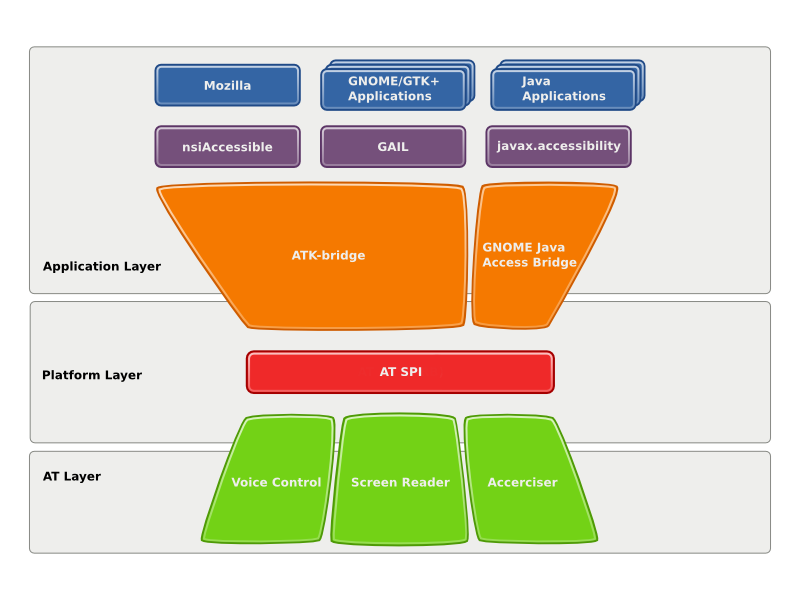
\includegraphics[height=0.5\linewidth]{images/a11y.png}
\caption{Akadálymentesített szoftverek elérése}
\label{fig:a11y}
\end{center}
\end{figure}

A működés modell (\ref{fig:a11y} ábra) végeredményben nem túl bonyolult. Az applikáció közvetlenül nem szólítható meg. Ahogy ezt hang alapú vezérlést megvalósító, illetve képernyőolvasó szoftverek is teszik, az \textit{AT SPI}-n (\textit{Assistive Technologies Service Provider Interface}) keresztül szólítják meg a megfelelő szoftvert. Amennyiben ez egy \textit{GTK+} felhasználásával fejlesztett alkalmazás, akkor a kérésre a \textit{Gail} (\ref{sec:gail}) nevű alrendszert futtatva válaszol, az \textit{ATK} interfészben leírtaknak megfelelően.
